\chapter{Elegant\LaTeX{} 系列模板介绍}

Elegant\LaTeX{} 项目组致力于打造一系列美观、优雅、简便的模板方便用户使用。目前由 \href{https://github.com/ElegantLaTeX/ElegantNote}{ElegantNote},\href{https://github.com/ElegantLaTeX/ElegantBook}{ElegantBook},\href{https://github.com/ElegantLaTeX/ElegantPaper}{ElegantPaper} 组成,分别用于排版笔记,书籍和工作论文。强烈推荐使用最新正式版本!本文将介绍本模板的一些设置内容以及基本使用方法。如果您有其他问题,建议或者意见,欢迎在 GitHub 上给我们提交 \href{https://github.com/ElegantLaTeX/ElegantBook/issues}{issues} 或者邮件联系我们。

我们的联系方式如下,建议加入用户 QQ 群提问,这样能更快获得准确的反馈,加群时请备注 \LaTeX{} 或者 Elegant\LaTeX{} 相关内容。
\begin{itemize}
  \item 官网:\href{https://elegantlatex.org/}{https://elegantlatex.org/}
  \item GitHub 网址:\href{https://github.com/ElegantLaTeX/}{https://github.com/ElegantLaTeX/}
  \item CTAN 地址:\href{https://ctan.org/pkg/elegantbook}{https://ctan.org/pkg/elegantbook}
  \item 文档 Wiki:\href{https://github.com/ElegantLaTeX/ElegantBook/wiki}{https://github.com/ElegantLaTeX/ElegantBook/wiki}
  \item 下载地址:\href{https://github.com/ElegantLaTeX/ElegantBook/releases}{正式发行版},\href{https://github.com/ElegantLaTeX/ElegantBook/archive/master.zip}{最新版}
  \item 微博:Elegant\LaTeX{}
  \item 微信公众号:Elegant\LaTeX{}
  \item 用户 QQ 群:692108391 
  \item 邮件:\email{elegantlatex2e@gmail.com}
\end{itemize}


\section{ElegantBook 更新说明}

此次为 3.x 最后一个版本,在 3.10 基础上,主要为了解决 \TeX{} Live 2020 中编译错误,具体内容有:

\begin{enumerate}
  \item \textbf{重要修正}:修复因为 \lstinline{gbt7714} 宏包更新导致的 \lstinline{natbib option clash} 错误;
  \item 由于 \lstinline{pgfornament} 宏包未被 \TeX Live 2020 收录,因此删除 base 相关的内容;
  \item 修复部分环境的空格问题;
  \item 增加了意大利语言选项 \lstinline{lang=it}。
\end{enumerate}

\begin{note}
如果你使用旧版本切换到新版本时,遇到问题时,请核对文档中是否有 \lstinline{pageanchor} 字样。如果有,请删除文档中的 \lstinline|\hypersetup{pageanchor=true}|,并且在 \lstinline{\maketitle} 和 \lstinline{\tableofcontents} 之间添加 \lstinline{\frontmatter}。2.x 版本的用户请仔细查看\href{https://github.com/ElegantLaTeX/ElegantBook/wiki/convert}{跨版本转换}。
\end{note}

\section{模板安装与更新}

你可以通过免安装的方式使用本模板,包括在线使用和本地(文件夹内)使用两种方式,也可以通过 \TeX{} 发行版安装使用。

\subsection{在线使用模板}

我们把三套模板全部上传到 \href{https://www.overleaf.com/}{Overleaf} 上了,网络便利的用户可以直接通过 Overleaf 在线使用我们的模板。使用 Overleaf 的好处是无需安装 \TeX{} Live 2020,可以随时随地访问自己的文件。查找模板,请在 Overleaf 模板库里面搜索 \lstinline{elegantlatex} 即可,你也可以直接访问\href{https://www.overleaf.com/latex/templates?addsearch=elegantlatex}{搜索结果}。选择适当的模板之后,将其 \lstinline{Open as Template},即可把模板存到自己账户下,然后可以自由编辑以及与别人一起协作。更多关于 Overleaf 的介绍和使用,请参考 Overleaf 的\href{https://www.overleaf.com/learn}{官方文档}。

\begin{remark}
Overleaf 上,中文需要使用 \hologo{XeLaTeX} 进行编译,英文建议使用 \hologo{pdfLaTeX} 编译。
\end{remark}

\subsection{本地免安装使用}


\textbf{免安装}使用方法如下,从 GitHub 或者 CTAN 下载最新(正式)版文件,严格意义上只需要类文件 \lstinline{elegantbook.cls}。然后将模板文件放在你的工作目录下即可使用。这样使用的好处是,无需安装,简便;缺点是,当模板更新之后,你需要手动替换 \lstinline{cls} 文件。

\subsection{发行版安装使用}

如果你是 \TeX{} Live 2019 用户,我们推荐你直接进行安装和更新。你可以通过 \TeX{} Live 2019 自带的 \lstinline{tlshell}\footnote{也叫 \TeX{} Live Manager} 进行安装。安装非常简单,步骤如下,搜索并打开 \lstinline{tlshell},然后通过 \lstinline{File -> Load Default Repository} 加载远程仓库,如果你不想使用默认的仓库,你可以通过 \lstinline{Options} 下的菜单设置远程仓库。设置好仓库之后,等待仓库加载完毕,你可以在下面的搜索栏搜索 \lstinline{elegantbook},然后选择进行安装与更新。

\begin{figure}[htbp]
  \centering
  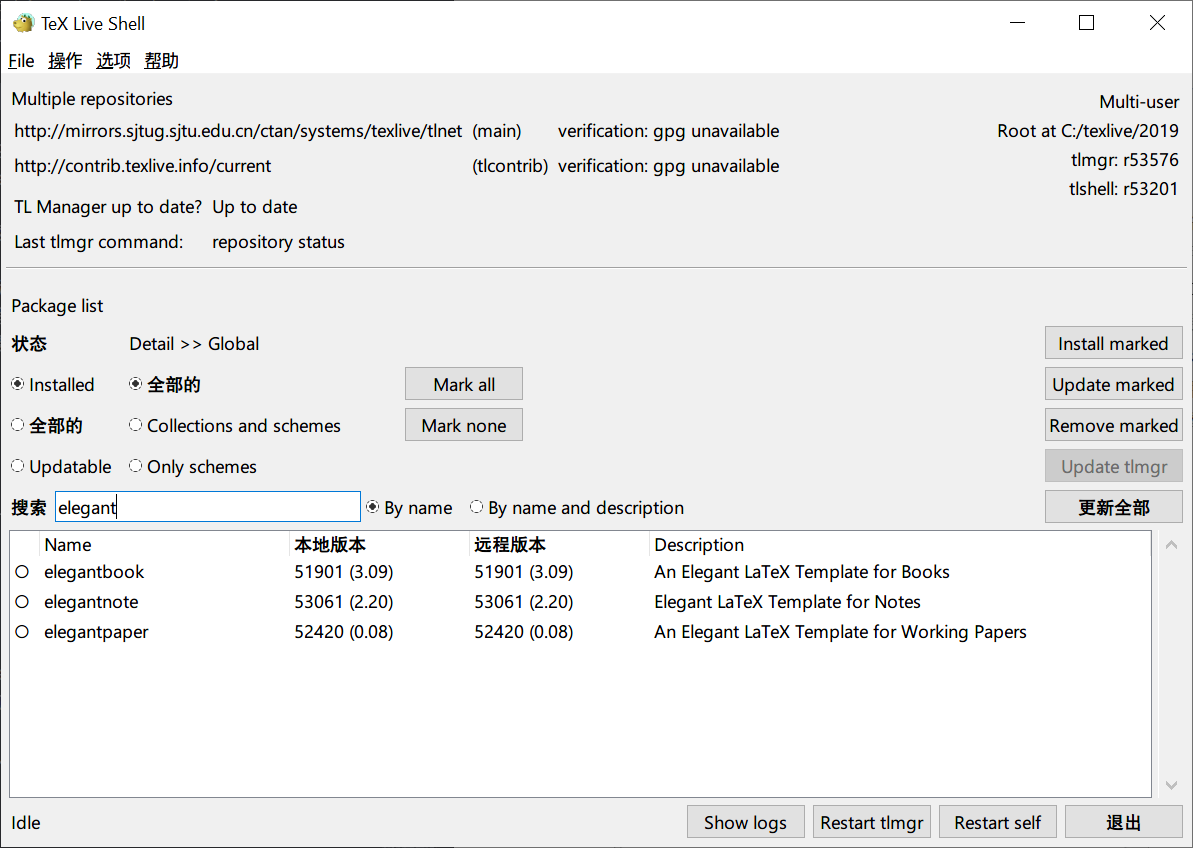
\includegraphics[width=0.7\textwidth]{tlshell.png}
  \caption{使用 \TeX{} Live Shell 安装 ElegantBook 模板}
\end{figure}

\subsection{更新问题}

如果使用 \lstinline{tlshell} 无法更新模板,请使用命令行全部更新全部宏包或者使用免安装的方法使用本模板。

通过命令行(管理员权限)输入下面的命令对 tlmgr 自身和全部宏包进行更新。

\begin{lstlisting}
  tlmgr update --self 
  tlmgr update --all
\end{lstlisting}

更多的内容请参考 \href{https://tex.stackexchange.com/questions/55437/how-do-i-update-my-tex-distribution}{How do I update my \TeX{} distribution?}

\subsection{其他发行版本}

如果你是 \TeX{} Live 2018 的用户,由于 2018 难以更新到 2019,建议卸载 2018 重装 2019。如果嫌麻烦,你可以手动安装模板,将 \lstinline{elegantbook.cls} 复制到你的 \TeX{} Live 目录下,默认安装目录为 \lstinline|C:\texlive\2019\texmf-dist\tex\latex\elegantbook|,然后通过命令行(管理员权限),运行 \lstinline{texhash} 即可。

由于宏包版本问题,本模板不支持 C\TeX{} 套装。更多关于 \TeX{} Live 2019 的安装使用以及 C\TeX{} 与 \TeX{} Live 的兼容、系统路径问题,请参考官方文档以及啸行的\href{https://github.com/OsbertWang/install_latex/releases}{一份简短的安装 \LaTeX{} 的介绍}。


\section{用户作品计划}

Elegant\LaTeX{} 系列模板从创立至今已经有 9 年了,我们的模板也受到了很多用户的喜爱,在此,为了促进模板用户之间的交流,了解用户需求,完善本模板,我们将建立一个区域专门展示用户的文档,包括但不限于 GitHub 和官网等。如果你愿意将自己的作品展示出来,请邮件或者其他方式联系我们。如果自己代码已经传到 GitHub 或者 Gitee 等网站,可以提供对应网址。\href{https://github.com/ElegantLaTeX/Archive/tree/master/Collections}{用户文档中心}目前有下面一些作品:
\begin{enumerate}
\item 唐绍东:微积分笔记
\item 曲豆豆:超甜微积分习题集
\item 王世强:《化工数值计算与 MATLAB》复习指南
\item 李晨迪:Fluid Mechanics Notes
\item 肖明顺:地球物理勘查常用规范汇编
\item 白衣卿相:期末复习笔记-拓扑学摘要
\end{enumerate}

\section{关于提交}

出于某些因素的考虑,Elegant\LaTeX{} 项目自 2019 年 5 月 20 日开始,\textbf{不再接受任何非作者预约性质的提交}(pull request)!如果你想改进模板,你可以给我们提交 issues,或者可以在遵循协议(LPPL-1.3c)的情况下,克隆到自己仓库下进行修改。

\section{协作人员招募}

招募 Elegant\LaTeX{} 的协作人员(志愿者),没有报酬。工作内容:翻译 Elegant\LaTeX{} 系列模板文档,维护模板的维基,如果有公众号文稿写作经历的话,也可以帮忙写微信稿。本公告长期有效。目前 Elegant\LaTeX{} 共有 4 名协作人员,在此感谢他们无私的奉献!
\begin{itemize}
  \item 官方文档翻译: \href{https://github.com/peggy2006xzyz}{YPY};
  \item GitHub 维基维护: \href{https://github.com/izinngo}{Ingo Zinngo}、\href{https://github.com/xiaohao890809}{追寻原风景};
  \item QQ 群管理、FAQ 整理: \href{https://github.com/sikouhjw}{Sikouhjw}.
\end{itemize}

另外,也感谢 \href{https://github.com/stone-zeng}{Xiangdong Zeng}、\href{https://github.com/latexers}{逐鹿人}等人帮忙群管理。

\section{致谢}
2019 年 5 月 20 日,ElegantBook 模板在 GitHub 上的收藏数(star)达到了 100\footnote{截止 3.10 版本正式发布,star 数为 374。}。在此特别感谢 China\TeX{} 以及 \href{http://www.latexstudio.net/}{\LaTeX{} 工作室}对于本系列模板的大力宣传与推广。\LaTeX{} 工作室网站上有很多精彩的帖子和精致的模板,欢迎大家去挖掘里面的宝藏,这也是国内最全面的 \LaTeX{} 相关的网站。

如果你喜欢我们的模板,你可以在 GitHub 上收藏我们的模板。
%\begin{figure}[htbp]
%  \centering
%  \includegraphics[width=\textwidth]{star.png}
%  \caption{一键三连求赞}
%\end{figure}

\section{捐赠}

如果您非常喜爱我们的模板或者我,你还可以选择捐赠\footnote{最好在捐赠时备注信息。}以表达您对我们模板和我的支持。本模板自 3.08 版本发布了捐赠信息之后,收到了超过 1500 元的捐赠(四舍五入就是一个亿),非常感谢!

\begin{figure}[htbp]
\centering

\includegraphics[width=0.5\textwidth]{donate.jpg}
\end{figure}

\textbf{赞赏费用的使用解释权归 Elegant\LaTeX{} 所有,并且不接受监督,请自愿理性打赏}。10 元以上的赞赏,我们将列入捐赠榜,谢谢各位金主!

\begin{table}[!htb]
  \centering
  \caption{Elegant\LaTeX{} 系列模板捐赠榜}
    \begin{tabular}{*{4}{>{\scriptsize}c}|*{4}{>{\scriptsize}c}}
    \hline
    \textbf{捐赠者} & \textbf{金额} & \textbf{时间} & \textbf{渠道} & \textbf{捐赠者} & \textbf{金额} & \textbf{时间} & \textbf{渠道} \\
    \hline
    Lerh  & 10 RMB & 2019/05/15 & 微信    & 越过地平线 & 10 RMB & 2019/05/15 & 微信 \\
    银桑    & 20 RMB & 2019/05/27 & 微信    & *空    & 10 RMB & 2019/05/30 & 微信 \\
    latexstudio.net & 666 RMB & 2019/06/05 & 支付宝   & A*n   & 40 RMB & 2019/06/15 & 微信 \\
    * 夏   & 22 RMB & 2019/06/15 & 微信    & * 倩   & 21 RMB  & 2019/06/15 & 微信 \\
    Cassis & 11 RMB & 2019/06/30 & 微信    & *君    & 10 RMB & 2019/07/23 & 微信 \\
    P*u   & 50 RMB & 2019/07/30 & 微信    & *萌    & 19 RMB & 2019/08/28 & 微信 \\
    曲豆豆   & 10 RMB & 2019/08/28 & 微信    & 李博    & 100 RMB & 2019/10/06 & 微信 \\
    Njustsll & 10 RMB & 2019/10/11 & 微信    & 刘志阔   & 99.99 RMB & 2019/10/15 & 支付宝 \\
    * 韬   & 16 RMB & 2019/10/17 & 微信    & 赤霓    & 12 RMB & 2019/10/17 & 支付宝 \\
    追寻原风景 & 10 RMB & 2019/10/28 & 微信    & 郭德良   & 88 RMB & 2019/11/03 & 微信 \\
    自强不息  & 20 RMB & 2019/11/04 & 支付宝   & 读书之虫  & 20 RMB & 2019/11/18 & 微信 \\
    *等    & 10 RMB & 2019/11/18 & 微信    & *哲    & 20 RMB & 2019/11/18 & 微信 \\
    佚名    & 10 RMB & 2019/11/24 & 微信    & Jiye Qian & 66 RMB & 2019/12/04 & 微信 \\
    * 阳   & 20 RMB & 2019/12/05 & 微信    & Catcher & 11 RMB & 2019/12/08 & 支付宝 \\
    希尔波特门徒 & 10 RMB & 2019/12/09 & 支付宝   & * 伟   & 10 RMB & 2019/12/09 & 微信 \\
    Simon & 20 RMB & 2019/12/11 & 支付宝   & 流殇丶浅忆 & 66.60 RMB & 2019/12/18 & 支付宝 \\
    羽     & 10 RMB & 2019/12/20 & 支付宝   & * 琛   & 15 RMB & 2019/12/20 & 微信 \\
    随风    & 20 RMB & 2019/12/27 & 支付宝   & Ws    & 23.30 RMB & 2019/12/28 & 微信 \\
    初八    & 100 RMB  & 2020/01/02 & 支付宝   & p*e   & 20 RMB & 2020/01/03 & 微信 \\
    Shunmx & 100 RMB & 2020/01/03 & 微信    & hj    & 10 RMB & 2020/01/03 & 微信 \\
    F*5   & 10 RMB & 2020/01/03 & 微信    & S*m   & 20.20 RMB & 2020/01/03 & 微信 \\
    二代青雉  & 13 RMB & 2020/01/14 & 支付宝   & *?    & 66 RMB & 2020/01/15 & 微信 \\
    Mr. Xiong & 20 RMB & 2020/01/17 & 微信    & *博    & 15 RMB & 2020/01/18 & 微信 \\
    * 者  & 10 RMB & 2020/02/02 & 微信    & Jackie  &  88.80 RMB  &  2020/02/09 & 微信 \\
    Henry\_Sun、 & 50 RMB & 2020/02/14 & 支付宝 & * 桥  & 50 RMB & 2020/02/21 & 微信 \\
    昀琏 & 10 RMB & 2020/03/02 & 支付宝 & S*y  &  10 RMB  &  2020/03/15 & 微信 \\
    * 哥  & 66.66 RMB & 2020/03/17 & 微信    &   K*e & 30 RMB & 2020/03/30 & 微信\\
    * 阳  &  20 RMB  &  2020/04/02 & 微信 & 士*n  & 30 RMB & 2020/04/11 & 微信 \\
    \hline
    \end{tabular}%
  \label{tab:donation}%
\end{table}%

另外,为了表示感谢,我们制作了捐赠纪念证,欢迎大家来信告知邮箱以及姓名(艺名),我们将通过邮件发送电子版纪念证。

\begin{figure}[!htbp]
\centering
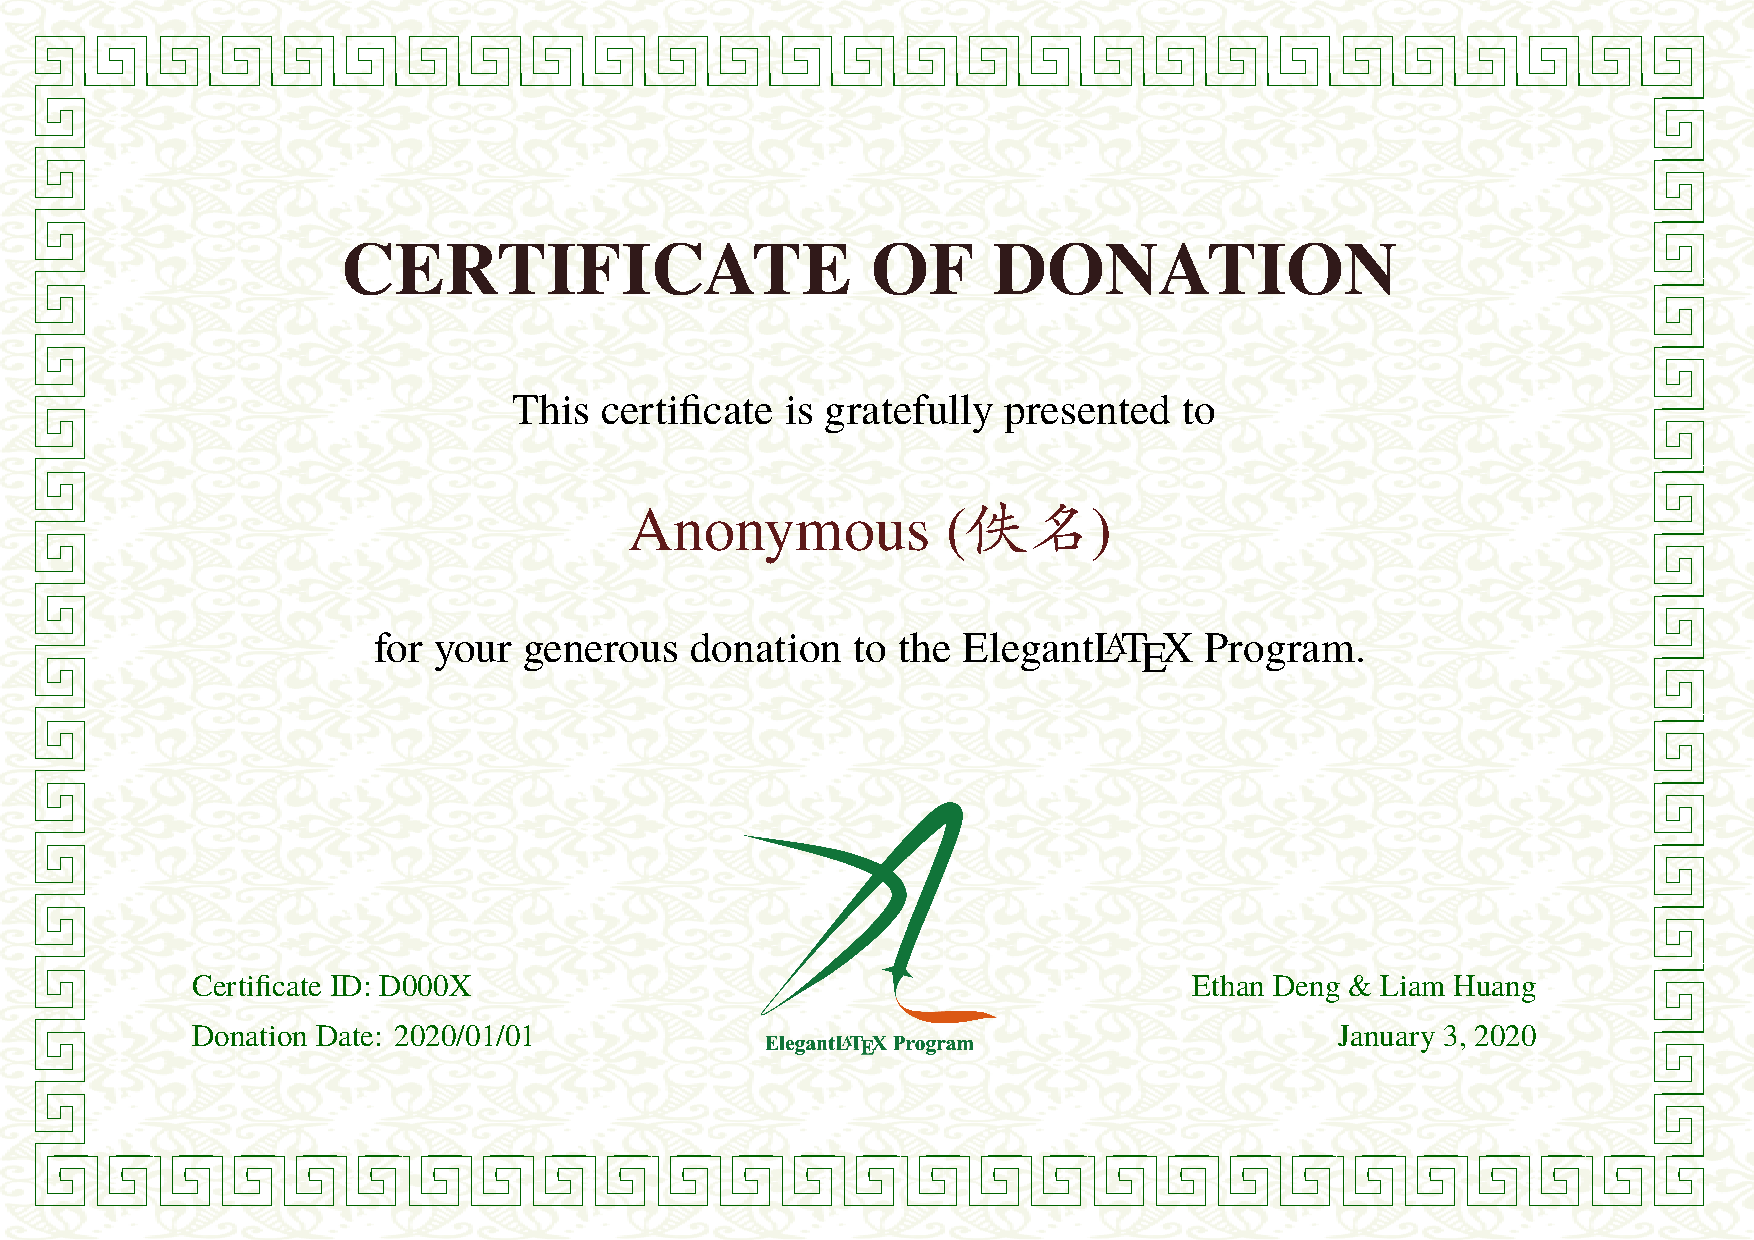
\includegraphics[width=0.6\textwidth]{cert.pdf}
\end{figure}
